\documentclass[UKenglish, final]{uiomasterbeta}  %% ... or norsk or nynorsk or USenglish
                                      %% ... add option 'final' to remove showkeys
\usepackage[utf8]{inputenc}           %% ... or latin1
\usepackage[T1]{url}\urlstyle{sf}
\usepackage{babel, csquotes, graphicx, textcomp, uiomasterfp, varioref}
\usepackage[backend=biber,
    sortcites  = true,
    giveninits = true,
    %doi = false,
    isbn = false,
    url = false,
   %sortlocale = nb_NO, %% ... known bug in biblatex - to be resolved
    citestyle=phys,
    style=phys]{biblatex} %% ... phys by AIP
    %% For alternatives, see https://www.overleaf.com/learn/latex/Bibtex_bibliography_styles
% \DeclareNameAlias{sortname}{family-given} 
% \DeclareNameAlias{default}{family-given} %% ... Wiles, A. instead of A. Wiles.
\usepackage[hidelinks]{hyperref}
\usepackage{kantlipsum}  
\usepackage{booktabs}
\usepackage{microtype}
\microtypesetup{protrusion = false}

\usepackage{physicspreamble}

\title{Nuclear excitation functions for medical isotope production}       %% ... or whatever
\subtitle{Targeted radionuclide therapy via $^{\text{nat}}\text{Zr}(d,x)^{86,88,90}\text{Y}$}         %% ... if any
\author{Elise Malmer Martinsen}                      %% ... or whoever 

\addbibresource{mybib.bib}            %% ... or whatever


\begin{document}
\uiomasterfp[dept={Department of Physics},  %% ... or your department
  program={Physics},                        %% ... or your study program
  % supervisor={Sunniva Siem, Andrew Voyles and \newline Kevin Ching Wei Li },                    %% ... or blank
  supervisors={Sunniva Siem \and Andrew Voyles \and Kevin Ching Wei Li},     %% if more than one
  master,                                   %% ... or bachelor
  long,                                      %% ... or short
  color=elise]                                 %%... color options  

\frontmatter{}
    \begin{abstract}
\markboth{}{} %% removes header from pages
\noindent

\todo[inline]{Add new section about results in \cref{p1:results}.}
\end{abstract}
     \begin{sammendrag}
\markboth{}{} %% removes header from pages
\noindent
Det skal være et sammendrag på norsk i Ph.d.-avhandlinger. Det er like greit å ha det i en masteroppgave også. Det kan være utfordrende å skrive, men det er nyttig.
\todo[inline]{Add new section about results in \cref{p1:results}}
\end{sammendrag}

\tableofcontents{}
\markboth{}{} %% removes header from pages
 \cleardoublepage
\listoftables
\addcontentsline{toc}{chapter}{List of Tables}
\markboth{}{}  %% removes header from pages
\listoffigures
\addcontentsline{toc}{chapter}{List of Figures}
\markboth{}{} %% removes header from pages

  \begin{preface}
\addcontentsline{toc}{chapter}{Preface}  
\markboth{}{} %% removes header from pages
\todo[noline]{Rewrite this.}

\end{preface}
  % \cleardoublepage %% May need this if longer than one page
  %\chapter{Acknowledgements}
\begin{acknowledgements}
\addcontentsline{toc}{chapter}{Acknowledgements}  
\markboth{}{} %% removes header from pages

\end{acknowledgements}
  % \cleardoublepage %% May need this if longer than one page

\mainmatter{}

\part{Introduction}                   %% ... Innledning or Innleiing
\label{intro}
\begin{refsection}
    \chapter{Introduction}
\label{c:intro}


Letters in math mode will always be in math font, so you must specify text $x=2 and x=3$ is different from $x=2 \text{ and } x=3$. Notice the differential - and use whichever version you are comfortable with.
You can cleverly refer to your equation with \texttt{\textbackslash cref}: \cref{{eq:integration}}.

\section{Figures and Tables}

% Tikzfigure with \input:
\begin{figure}[htbp]
    \centering
    %\documentclass[tikz]{standalone}
%\begin{document}
    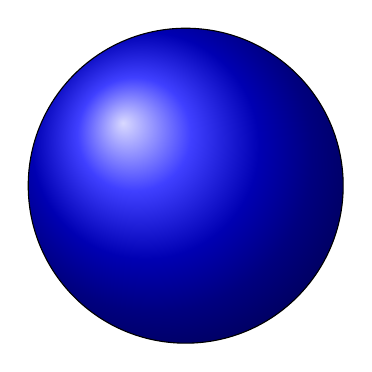
\begin{tikzpicture}
          \draw[shading = ball] (0, 0) circle (2);
    \end{tikzpicture}
%\end{document}
    \caption[One ball]{One ball - and the caption goes underneath the figure.}
\end{figure}

% Includegraphics
\begin{figure}[thbp]
    \centering
    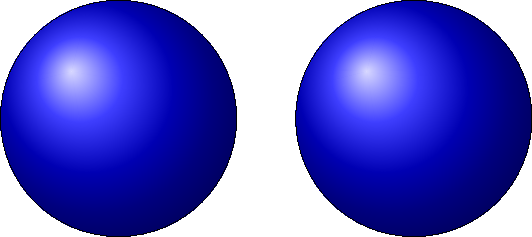
\includegraphics{figures/balls.pdf}
    \caption[Two balls]{Two balls.}
\end{figure}

% Todonotes:
\begin{figure}[hbp]
    \centering
    \missingfigure{Three balls.}
    \caption[Three balls]{Three balls.}
\end{figure}


% Booktabs:
\begin{table}[htbp]
    \centering
       \caption[Colons (to appear in TOC)]{Caption above tables. Proper colon usage.}
    \begin{tabular}{@{}ll@{}}
        \toprule
        \textsf{Correct}               & \textsf{Incorrect}      \\
        \midrule
        \( \varphi \colon X \to Y \)   & \( \varphi : X \to Y \) \\[0.5ex]
        \( \varphi(x) \coloneqq x^2 \) & \( \varphi(x) := x^2 \) \\
        \bottomrule
    \end{tabular}
\end{table}

\begin{table}[htbp]
    \centering
    \caption[Arrows]{Proper arrow usage.}
    \begin{tabular}{@{}ll@{}}
        \toprule
        \textsf{Correct}     & \textsf{Incorrect}         \\
        \midrule
        \( A \implies B \)   & \( A \Rightarrow B \)      \\
        \( A \impliedby B \) & \( A \Leftarrow B \)       \\
        \( A \iff B \)       & \( A \Leftrightarrow B \)  \\
        \bottomrule
    \end{tabular}
    
\end{table}

% Tablefootnote and multirow:
\begin{table}[!ht]
   \caption[Dashes]{Proper dash usage.}
    \centering
    \begin{tabular}{@{}ll@{}}
        \toprule
        \textsf{Correct}
        & 
        \textsf{Incorrect}
        \\
        \midrule
        \( -1 \) 
        & 
        -1
        \\[0.3ex]
        1--10
        &
        1-10
        \\[0.3ex]
        Birch--Swinnerton-Dyer\tablefootnote{It is now easy to tell that Birch and Swinnerton-Dyer are two people, but I don't know why the footnote lands on the wrong page.} conjecture
        &
        Birch-Swinnerton-Dyer conjecture
        \\[0.3ex]
        The ball \dash which is blue \dash is round.
        &
        \multirow{ 2}{*}{The ball - which is blue - is round.}
        \\[0.3ex]
        The ball---which is blue---is round. 
        &
        \\
        \bottomrule
    \end{tabular}
  
\end{table}


\begin{table}[hbtp]
      \caption[Quotation marks]
    {Proper quotation mark usage.
    The \texttt{\textbackslash enquote} command chooses the correct
    quotation marks for the specified language. Moreover, \texttt{\textbackslash resizebox} has been used to control table width.}
    \centering
     \resizebox{\linewidth}{!} {
      \begin{tabular}{@{}*{2}{p{0.5\textwidth}}@{}}
           \toprule
        \textsf{Correct} &  \textsf{Incorrect}
        \\
        \midrule
        \enquote{This is an \enquote{inner quote} inside an outer quote}
        &
        'This is an "inner quote" inside an outer quote'
        \\
        \bottomrule
    \end{tabular}
    }
\end{table}

\section{Outline}

The rest of the text is organised as follows. See more lists in \cref{p1:discussion}.
\begin{description}
    \item[\cref{intro}] consists of an interesting introduction. You could consider calling this a chapter, not a part, but be aware of how this will affect numbering and the table of contents.
    \item[\cref{p1}] is all about your first research problem. The part is subdivided into an IMRaD-structure, starting with \cref{p1:intro}. 
    \item[\cref{p2}] is all about your second research problem. Perhaps you want to reset chapter numbering for each part, but then what would you do with the introduction and conclusion - and how would you ensure unique cross references? See \cref{p1} \cref{p1:intro}.
    \item[\cref{conc}] is your fabulous conclusion. Is this a part? Probably not. But then again you need to think very carefully about numbering.
\end{description}

   %    \printbibliography[heading=bibintoc,title={References}]
\end{refsection}

\part{First research problem}                    %% ... or ??
\label{p1}
    \begin{refsection} % empty pages are removed with 'final'
    \chapter{Introduction}
\label{p1:intro}
\section{Background}

\section{Research question}

\section{Data management plan}

    \chapter{Theory}
\label{theory}
\section{Half-life}
In the research of finding radionuclides that can be used in medical applications like targeted radionucleide therapy, brachytherapy and PET-scans one have to look at the properties of the nuclides. One of the most important properties is the effective half-life, which is the net half-life when considering both the physical half-life and the biological half-life \cite{yeongTherapeuticRadionuclidesNuclear2014a}.

\subsection{Physical half-life}
The physical half-life is the time it takes before half of the radionuclides have disintegrated. Radionucleides used in medical application can not have a short half-life as we need time to produce the radionucleides and separate it from other nuclei produced in the same reaction. In addition, if the radionuclides are not produced at the hospitals, we need an amount of time for transportation. The nuclei also require some time from it is injected into the patient until it has reached the cancer cells or the organs we would like to investigate. 
\vspace{3mm}
\\
On the other hand, a too long physical half-life is also not optimal as the patient will have radioactive nuclei in the body for a longer time, and expose surrounding people. To limit the dose for surrounding people, one would have to isolate the patient for a longer time period. This would make the treatment more expensive and will be a bigger burden for the patient. An ideal range for the physical half-life for radionucleides used in medical applications is between $6$ h and $7$ d \cite{yeongTherapeuticRadionuclidesNuclear2014a}.

\subsection{Biological half-life}
The biological half-life is defined as the time it takes for the body to get rid of half of the radionuclides and depends on the tracer used. If the biological half-life is long the physical half-life should not be too long as discussed above. A short biological half-life on the other hand, could open for the use of longer lived radionucleides as the nuclei will be emitted form the body and prevent the need for a long isolation period. However, if the biological half-life is too short, the nuclei will be submitted from the body with a high activity. Hence, extra conciderations regarding the waste management would be needed \cite{yeongTherapeuticRadionuclidesNuclear2014a}.



\section{Stopping power and linear energy transfer (LET)}
Biologisk effekt og at vi ønsker høy LET, men kort range osv. Enten her eller i brachytherapy section må jeg få med at beta fungerer bra pga range

\section{Brachytherapy}
When treating cancer today, we have many different options to choose from, like surgery, external radiation therapy, chemotherapy and targeted radiotherapy. Brachytherapy is another commonly used treatment method, and uses capsuled radioavtive sources. These sealed sources are placed right next to or in the tumor. Usually, the radioactive sources are removed from the body after the radionuclides have delivered the required dose. How much time is needed to deliver the required dose, depends on the the radionuclies and tumor, and will therefore be determined individually for every patient. However, the radioactive source is not always removed. Implants consisting of $^{125}$I can be placed inside the prostate gland, and is an example of a source that is left in the body and will give a dose to the canserous tissue during all the time they are active. Brachytherapy is frequently used to treat gynecological, breast, prostate and skin cancer, as well as some head and neck tumors and soft tissue sarcomas cite (https://www.iaea.org/topics/cancer-treatment-brachytherapy accsessed 27.04.23).



\section{PET-scans}
Historie
\vspace{3mm}
\\
hva er pet? annihilation, 
\vspace{3mm}
\\
applications, hvilke isotoper avhenger av prosess



\section{My ytrium isotope}

\section{Production of radionuclides}
\section{Nuclear reactions}
constarints (Q-value)


    \chapter{Stopping power}
\label{p1:stoppingpower}

\section{Stopping power calculations}
The aim of this part of the project was to improve the parameters used in the Ziegler parameterization used to calculate stopping power for charged particles in different materials. The Ziegler parameterization is from the 1970s and is a semi empirical model where some parameters were fitted to all the data available in the 1970s. A lot of new data has been collected since the model was made, and therefore we wanted to use all the stacked target measurements obtainable to make a new and improved fit of the parameters in the Ziegler model.  

\subsection{Energy determination}
To calculate the stopping power, we need to determine the energies of the different foils in all the stacked target experiments. The energies of the foils are already given in the published articles, but we want to determine the energies our self. The reason for this, is that most of the codes used to determine the energies listed in the articles are using the Ziegler parameterization. To avoid a circular argument, we therefore want to use other methods which don't use the Zielger model to find the energies. 
\vspace{3mm}
\\
The method we chose to determine the energies of the foils is called the Isotope cross section method. In this method we use the IAEA database to plot the ratio of the cross sections for two different monitor reactions that are seen in the same foil. We also plot the cross section ratios of the monitor reactions given by
\begin{equation}
    \frac{\sigma}{\sigma'} = \frac{A_0 / (1-\exp{-\lambda \Delta_{t_irr}})}{A_0' / (1-\exp{-\lambda' \Delta_{t_irr}})} = \frac{A_0(1-\exp{-\lambda' \Delta_{t_irr}})}{A_0' (1-\exp{-\lambda \Delta_{t_irr}})}
\end{equation}

where lalalalal.
The energy of a foil is then given by the crossing point of the IAEA ratio and the experimental cross section ratio. 
\vspace{3mm}
\\
The uncertainty of the calculated cross section ratios are calculated from the measurement uncertainties of the radiation time and the end of beam activities. 

\subsection{Calculating the stopping power}
After the energy in all the monitor foils is calculated, we can determine the stopping power given by
\begin{equation}
    S = -\frac{\Delta E}{\Delta x}
\end{equation}
where $\Delta E$ is the energy difference between the two foils and $\Delta x$ is the length between the two energy points. There is some uncertainty associated with the $\Delta x$ as it is not clear exactly where in the foils the energies we measure are. The monitor foils have a given thickness, and therefore we somehow have to determine which position in the foils corresponds to the energies determined. As a starting point we assumed that the energy of a foil corresponds to the middle of the foil. $\Delta x$ is therefore half of the thickness of the first monitor foil plus half of the thickness of the other monitor foil added with the thickness of the other foils and degraders in between the monitor foils, if any. 
\vspace{3mm}
\\
This method did not work as well as we expected. The stopping power values we got did not agree with our expectations, and we even got some negative values for the stopping power. The reason for this, is that the uncertainty in our energy calculations had big uncertainties. For some foils the uncertainty in energy was bigger than the difference in energy between the foil and the neighboring foil in the stack.











    \chapter{Experimental setup}
\label{experimental}
Summarize the chapter: what is described in the different sections?


\section{The stacked target activation method}
\section{Lawrence Berkeley National Laboratory's 88 Inch Cyclotron}
\section{Stack design}


\begin{table}[h!]%[htbp]
    \centering
    \label{Tab:foilcharacterization}
       \caption[Foil characterization]{The table shows the characteristics of each foil and the calculated areal densities. All lengths are measured in mm and masses are measured in g. The areal densities are given in mg/cm$^2$. The foils are listed in the same order they were irradiated and the horizontal lines divide the foils into compartments.}
    \begin{tabular}{lccccc}
        \toprule
        \textsf{Foil} & \textsf{Length} & \textsf{Width} & \textsf{Thickness} & \textsf{Mass} &  \textsf{Areal density}      \\
         & \textsf{(g)} & \textsf{(mm)} & \textsf{(mm)} & \textsf{(mm)}  & \textsf{(mg/cm$^2$)}      \\
        \midrule
        SS  & & & & &  \\
        \midrule
        Ni01  & $25.290$ & $25.005$ & $0.030$ & $0.147$ & $23.253$  \\
        Zr01  & $24.725$ & $24.993$ & $0.025$ & $0.100$ & $16.142$  \\
        Ti01  & $24.178$ & $25.190$ & $0.026$ & $0.070$ & $11.535$  \\
        Al (E1)  & $66.896$ & $66.662$ & & $3.046$ &  $68.312\pm0.071$\\
        Al (E2)  & $66.896$ & $66.662$ & & $3.043$  & $68.245\pm0.071$  \\
        \midrule
        Ni02  & $25.030$ & $25.243$ & $0.030$ & $0.146$ & $23.103$  \\
        Zr02  & $24.853$ & $25.550$ & $0.026$ & $0.104$ & $16.378$  \\
        Ti02  & $24.405$ & $24.520$ & $0.027$ & $0.070$ & $11.739$  \\
        Al (E3)  & $66.896$ & $66.662$ & & $3.048$ & $68.349\pm0.071$  \\
        \midrule
        Ni03  & $25.033$ & $25.115$ & $0.029$ & $0.145$ & $23.064$ \\
        Zr03  & $25.015$ & $24.768$ & $0.026$ & $0.100$ & $16.195$  \\
        Ti03  & $24.553$ & $25.200$ & $0.026$ & $0.070$ & $11.273$  \\
        \midrule
        Ni04  & $25.153$ & $25.190$ & $0.029$ & $0.147$ & $23.201$  \\
        Zr04  & $25.503$ & $24.758$ & $0.026$ & $0.102$ & $16.195$  \\
        Ti04  & $25.185$ & $25.223$ & $0.026$ & $0.071$ & $11.098$  \\
        \midrule
        Ni05  & $25.028$ & $25.120$ & $0.028$ & $0.143$ & $22.746$  \\
        Zr05  & $25.283$ & $24.698$ & $0.026$ & $0.099$ & $16.178$  \\
        Ti05  & $25.343$ & $24.755$ & $0.026$ & $0.071$ & $11.317$  \\
        \midrule
        SS & & & & & \\
        \bottomrule
    \end{tabular}
\end{table}
\section{HPGe detectors}
\section{Gamma-ray spectroscopy}
\subsection{Energy and peak shape calibration}
To find the corresponding energy for each channel number, energy calibration had to be done. The calibration point sources $^{133}$Ba ($t_{1/2} = XXX \pm$), $^{137}$Cs ($t_{1/2} = XXX \pm $), $^{56}$Co ($t_{1/2} = XXX \pm $) and $^{152}$Eu ($t_{1/2} = XXX \pm$) were used in this calibration, and can be seen in figure XXX. This sources have peaks with well known energies and are standard calibration sources for HPGe detectors. The gamma lines which were used in the calibration is listed in table XXX. 
\vspace{3mm}
\\
The detectors were calibrated at every distance the targets were counted. Unfortunately, not all the calibration sources were counted in every distance the targets were counted, but the $^{152}$Eu point source was measured at every distance. This calibration source alone has many well known energies, and can therefore be used for calibration alone. 
\vspace{3mm}
\\
For most HPGe detectors, including the ones used in this experiment, the relation between the energy and channel number is linear, and given by
\begin{equation}
    E = a + b\cdot C
\end{equation}
where $a$ is the intercept, $b$ is the slope of the line and $C$ is the channel number. The energy and peak shape calibration was done in Curie. 

\subsection{Efficiency calibration}
Intrinsic and geometric, every distance, write the formula 




\section{The irradiation}
The irradiation of the stacked targets was performed at the Lawrence Berkeley National Laboratory \todo{burde faktisk dobbeltsjekke dette} on the 13th of February 2017, and lasted for 20 minutes ($1200 \pm 3$ s). \todo{I just guessed the uncertainty} After the end of beam the foils were counted for five weeks. 
    \chapter{Analysis}
\label{analysis}


heihei
    \chapter{Results}
\label{p1:results}

\section{My first great result}

\section{My second great result}

\section{My third great result}

    \chapter{Discussion}
\label{p1:discussion}

\section{All my great results}

    \printbibliography[heading=bibintoc,title={References}]
\end{refsection}

\part{Second research problem}                     %% ... or ??
\label{p2}
\todo[inline]{Work in progress! Need to ask supervisor about this!}
\begin{refsection}
  \include{}
 %    \printbibliography[heading=bibintoc,title={References}]
\end{refsection}

\part{Conclusion}
\label{conc}
\begin{refsection}
  \chapter{Synergy}
\label{c:conclusion}


 %    \printbibliography[heading=bibintoc,title={References}]
\end{refsection}

\backmatter{}
    \appendix % "Chapter" is renamed "Appendix"
    \begin{refsection}
    \part*{Appendices}
    \chapter{The First Appendix}
\label{sec:first-app}

\section{First Section}

\section{Second Section}

    \chapter{The Second Appendix}
\label{sec:second-app}

 %    \printbibliography[heading=bibintoc,title={References}]
\end{refsection}
\end{document}
